\documentclass[10pt,twocolumn,letterpaper]{article}

\usepackage{cvpr}
\usepackage{times}
\usepackage{epsfig}
\usepackage{graphicx}
\usepackage{amsmath}
\usepackage{amssymb}

% Include other packages here, before hyperref.
\usepackage{color}
\usepackage{subfig}
\usepackage{tabularx}
\usepackage{multirow}
\usepackage[abs]{overpic}
\usepackage{cite}
\usepackage{algorithm}
\usepackage{algorithmic}
\usepackage{wrapfig}
\usepackage{diagbox}

% If you comment hyperref and then uncomment it, you should delete
% egpaper.aux before re-running latex.  (Or just hit 'q' on the first latex
% run, let it finish, and you should be clear).
\usepackage[pagebackref=true,breaklinks=true,letterpaper=true,colorlinks,bookmarks=false]{hyperref}

%\cvprfinalcopy % *** Uncomment this line for the final submission

\def\cvprPaperID{614} % *** Enter the CVPR Paper ID here
\def\httilde{\mbox{\tt\raisebox{-.5ex}{\symbol{126}}}}

\graphicspath{{./Imgs/}}
\DeclareGraphicsExtensions{.pdf,.jpg,.png}
\newcommand{\figref}[1]{Fig.~\ref{#1}}
\newcommand{\tabref}[1]{Tab.~\ref{#1}}
\newcommand{\secref}[1]{Sec.~\ref{#1}}
\newcommand{\algref}[1]{Algorithm~\ref{#1}}
\newcommand{\equref}[1]{Equ. (\ref{#1})}
\newcommand{\parahead}[1]{\textbf{#1}}
\newcommand{\myPara}[1]{\vspace{.1in}\noindent\textbf{#1}}
\def\ie{\emph{i.e.~}}
\def\eg{\emph{e.g.~}}
\def\etc{\emph{etc}}
\def\etal{{\em et al.}}
\def\sArt{{state-of-the-art~}}
\def\conv{\emph{conv~}}
\newcommand{\todo}[1]{{\textcolor{red}{#1}}}

% Pages are numbered in submission mode, and unnumbered in camera-ready
\ifcvprfinal\pagestyle{empty}\fi
\begin{document}

%%%%%%%%% TITLE
\title{RefinedBox: Refining for Fewer and High-quality Object Proposals}

\author{Yun Liu$^1$ \quad Ming-Ming Cheng$^1$ \quad Shi-Jie Li$^1$
\quad Jia-Wang Bian$^1$ \quad Peng-Tao Jiang \quad Dacheng Tao$^2$ \\
$^1$Nankai University\quad\quad$^2$ The University of Sydney
}

\maketitle
%\thispagestyle{empty}


%%%%%%%%%%%%%%%%%%%%%%%%%%%%%%%%%%%%%%%%%%%%%%%%%%%%%%%%%%%%%%%%%%%%%%%%%%%%%%%
\begin{abstract}
%
% Object detection is a fundamental and widely used computer vision technique.
% Recently, object proposal generation has shown value for object
% detection by hypothesizing object locations.
% High-quality object proposals that provide highly accurate but relatively
% few candidates would greatly benefit object detection.
%
Recently, object proposal generation has shown value for various 
vision tasks, such as object detection, instance semantic segmentation,
multi-label image classification, and weakly supervised learning, by 
hypothesizing object locations.
%
We are motivated by the fact that many bottom-up proposal methods generate 
dense proposals to cover as many objects as possible but that 
(i) they usually fail to rank these proposals properly and 
(ii) the number of proposals is very large.
%
For example, the well-known object proposal generation methods, Edge Boxes
and Selective Search, can achieve high detection recall with thousands of
proposals per image.
But the large number of generated proposals causes subsequent analysis
difficult due to the large false alarms and heavy computation load.
%
To significantly reduce the number of proposals, we design a computationally
lightweight neural network to refine the initial object proposals.
The refinement consists of two parallel processes, re-ranking and box regression.
The proposed network can share convolutional features with other high-level 
tasks by joint training, so the proposal refinement can be very fast.
We show a joint training example of object detection in this paper.
%
Extensive experiments demonstrate that our method can achieve \sArt 
performance with a few proposals compared with the well-known proposal 
generation methods such as RPN, Selective Search, and Edge Boxes.
%The proposed object detection method also performs better than Faster R-CNN.
\end{abstract}


%%%%%%%%%%%%%%%%%%%%%%%%%%%%%%%%%%%%%%%%%%%%%%%%%%%%%%%%%%%%%%%%%%%%%%%%%%%%%%%
\section {Introduction}
%
% In the past few years, convolutional neural networks have driven a number of
% recent advances in object detection.
% % object detection has undergone a great development due to
% % the success of convolutional neural network.
% %
% The \sArt object detection methods can be grouped into two main classes:
% region-free methods \cite{redmon2016you,liu2016ssd}
% and region-based methods \cite{girshick2014rich,girshick2015fast,ren2015faster}.
% %
% The region-free methods seek to detect and recognize objects directly from natural images.
% This category of methods is very efficient while suffering the decline of accuracy.
% %
% The region-based methods have shown high accuracy on mainstream object detection
% benchmarks \cite{lin2014microsoft,pascal-voc-2007}.
% These methods usually produce object proposals first and then
% train deep models to classify these proposals.
% Thus proposal generation is very important for object detection because it provides
% the search space for follow-up classification.


% Object proposal generation aims to hypothesize object locations 
% without recognizing object categories.
% It has been widely used to reduce search spaces for many vision 
% applications including 
% object detection \cite{girshick2014rich,girshick2015fast},
% instance semantic segmentation \cite{he2017mask,arnab2017pixelwise},
% multi-label classification \cite{wei2016hcp},
% video summarisation \cite{lee2015predicting},
% and deep multiple instance learning \cite{wu2015deep}.
% %
% Typical proposal generation methods usually output a set of bounding 
% boxes and corresponding objectness scores that measure how likely 
% each box covers a complete object of any category.
% %
% The quality of predicted object proposals is usually measured by the 
% balance between detection recall and proposal number.
% A good proposal generation algorithm should cover most of the objects
% in an image with a small number of proposals.
% %
% In this paper, we focus on \emph{mining the number of proposals}
% while obtaining high detection recall.



\begin{figure}[!t]
	\centering
    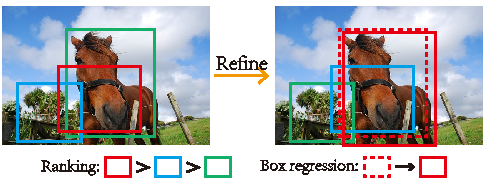
\includegraphics[width=\linewidth]{box_refinement}
    \caption{The overview of object proposal refinement.The left image shows the
    	original proposals, and the right image shows the results after refinement.
        We first re-rank the proposals by computing new objectness scores, after
        which a box regression procedure is applied to each proposal box for
        accurate location.}
    \label{fig:refinement_overview}
    \vspace{-0.2in}
\end{figure}


% Since object proposals will \todo{usually} be fed into object
% detection framework later,
% a good proposal method should produce a small number of proposals
% while covering as many objects in an image as possible.
%
Generating \emph{a small number of} object proposals while covering as
many objects in an image as possible is crucial for the efficiency
and accuracy of consequent high-level applications, such as 
object detection \cite{girshick2014rich,girshick2015fast},
instance semantic segmentation \cite{he2017mask,arnab2017pixelwise},
multi-label classification \cite{wei2016hcp},
video summarisation \cite{lee2015predicting},
and deep multiple instance learning \cite{wu2015deep},
by reducing the search space and false alarms.
%
Many object proposal methods have been developed such as Selective 
Search \cite{uijlings2013selective}, Edge Boxes \cite{zitnick2014edge}
and MCG \cite{arbelaez2014multiscale}.
However, these methods usually generate thousands of object proposals
per image, which is too many for many vision tasks
\cite{wei2016hcp,wu2015deep,qi2016augmented,li2016weakly}.
%
Recently, RPN \cite{ren2015faster}, a deep learning based proposal
method, has attracted a lot of attention in this field because it
can provide high detection recall with much fewer candidate boxes.
However, the number of true objects (\eg usually less than 10)
is still much smaller than the RPN proposals (\eg a few hundred).


Can we significantly reduce the number of proposals while maintaining
the high recall?
This is crucial for a much wider range of applications,
\eg mining knowledge from huge amounts of unlabeled/weakly-labeled
data \cite{wei2016hcp,wu2015deep},
for which the large number of false positives will pose significant challenges
not only for computational efficiency but also for system stability.
%
Some research towards reducing the number of proposals for specific 
vision tasks has been proposed.
%
For example, Wei \etal \cite{wei2016hcp} adopted normalized cut
\cite{shi2000normalized} to cluster bounding boxes generated by BING 
\cite{cheng2014bing} and picked out the top 1 hypothesis with the highest
objectness score in each cluster.
They applied the selected proposals to multi-label image classification
and achieved the \sArt performance.
%
Qi \etal \cite{qi2016augmented} introduced aggregation score at each pixel
by calculating the sum of all objectness scores whose corresponding
proposal boxes cover this pixel.
The resulting aggregation score maps are used to estimate object locations.
%
Li \etal \cite{li2016weakly} adopted a mask-out strategy to collect proposals
with higher quality for each object category.
A proposal is collected for one class if the mask-out image by this proposal 
box has a significant drop in classification score of this class.



%The small number of proposals is not only necessary for the efficiency
%of follow-up detection, but also necessary for the detection accuracy
%by reducing the false alarms.
%Usually, only several hundred proposals of RPN are sufficient to cover most
%of the objects in an image.
%%
%Can the quality of object proposals be further improved?
%The answer is yes.

In this paper, we focus on \emph{mining the number of proposals}
while obtaining high detection recall.
%
We observe that some bottom-up proposal generation methods can achieve high 
detection recall when the number of candidate boxes is sufficiently large.
Of course, the large number of candidates causes many false positives in
the subsequent applications and thus affects the final performances.
%
However, if we can select the good ones from the large set of candidates,
it will benefit a series of vision tasks.
%
Several algorithms have been proposed to refine object proposals,
including DeepBox \cite{kuo2015deepbox} and MTSE \cite{chen2015improving}.
DeepBox builds a neural network to recompute the objectness scores of the
initial boxes and then re-rank them.
MTSE tries to refine each box using superpixels by making each box tightly
cover some inner superpixels.
However, the proposal quality of DeepBox is worse than RPN, and thus
the number of proposals can not be reduced.
Besides, the performance of MTSE depends on the quality of superpixels,
and the image segmentation within MTSE causes a significant increase in
computational load.


We propose a novel method to re-rank and align existing proposal
boxes in a single inference of a neural network.
An overview of our approach is shown in \figref{fig:refinement_overview}.
Our refinement of candidate boxes includes two steps: re-ranking and box regression.
The re-ranking step tries to re-rank the proposals according to the
tightness of their coverage with complete objects.
The box regression step attempts to fine tune the shapes and locations of boxes
in order to make them cover real objects more tightly.
%
To achieve this goal, our refinement network is designed to learn new objectness
scores and performs box regression simultaneously.
The proposed network is also computationally lightweight,
so it can be applied to applications with a little extra time consumption.
The training process of refinement can be performed in an end-to-end manner.
%
For the sake of brevity, we call our proposed method \textbf{RefinedBox} 
in the remainder of this paper.
%
Since RefinedBox is lightweight and easily optimized, it has the potential
to share convolutional features with high-level applications by joint training.
To show a joint training example, we unify RefinedBox and the well-known 
detection framework of Fast R-CNN \cite{girshick2015fast} by connecting our 
refinement layers after the last convolutional layer of the base network
such as VGG16 \cite{simonyan2014very}.
We follow the alternating fine-tuning training used in Faster R-CNN.
As a result, our refinement network can share the base convolutional 
layers with the consequent object detection network, making the refinement 
procedure very efficient.


Using the proposal boxes produced by Edge Boxes \cite{zitnick2014edge} as input,
we train and test our network on the VOC2007 dataset \cite{pascal-voc-2007} using VGG16.
For object proposal generation, our method achieves the detection recall of
88.8\% and 78.8\% for intersection-over-union (IoU) 0.5 and 0.7,
respectively, using only 10 refined boxes per image.
Using only 10 boxes for object detection, our method achieves
a mean average precision (mAP) of 65.4\% compared with the mAP of 54.1\% 
for RPN \cite{ren2015faster}.
Thus, our proposed RefinedBox method can generate more accurate object
proposals than RPN when the proposal number is limited.


\begin{figure*}[!ht]
	\centering
    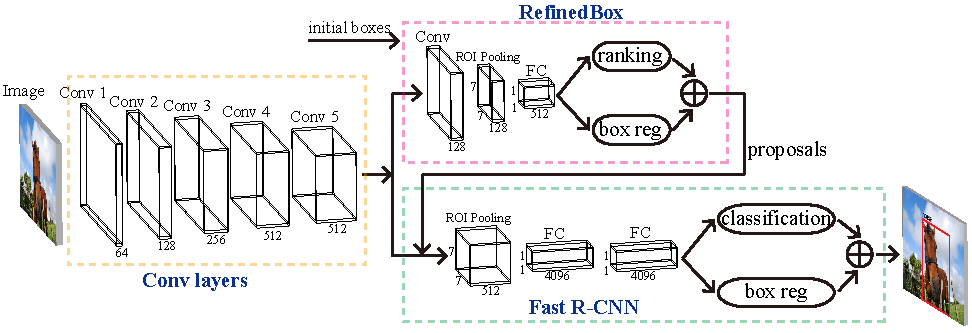
\includegraphics[width=\linewidth]{network}
    \caption{The overview of our network architecture. We display object detection as 
    	an example of joint training. The proposed network takes a nature image and
        corresponding initial boxes produced by other object proposal generation 
        methods such as Edge Boxes as input. The branch of RefinedBox is
        designed to refine the initial boxes, then the refined boxes are inputted into
        the branch of Fast R-CNN for classification. Note that the refinement of boxes
        and consequent object detection can share the convolutional features.}
    \label{fig:network}
    \vspace{-0.15in}
\end{figure*}


%%%%%%%%%%%%%%%%%%%%%%%%%%%%%%%%%%%%%%%%%%%%%%%%%%%%%%%%%%%%%%%%%%%%%%%%%%%%%%%
\section{Related Work}
%
Since this paper targets object proposal refinement, we first 
briefly describe recent developments in object proposal generation.
We then go on to discuss the refinement techniques of bounding boxes.
We broadly divide the related research into three parts: 
segmentation-based proposal generation methods, edge-based methods, 
and proposal post-processing methods.


% \myPara{Object detection} is a fundamental and widely used technique
% in computer vision.
% Object detection aims to detect all objects of interest in an image
% and recognize their categories.
% %
% With the great success of the convolutional neural networks (CNNs) on large
% scale object recognition tasks in recent years, more and more methods based
% on CNNs have been proposed \cite{girshick2014rich,girshick2015fast}.
% These object detection methods can be broadly divided into two groups:
% region-based methods and region-free methods.
% %
% The region-based methods divide this task into two steps of object proposal
% generation and the post-classification of these proposals.
% R-CNN \cite{girshick2014rich} is the first method that uses semantic information
% in neural networks to classify object proposals.
% Then, some of its variants were proposed, including
% SPPNet \cite{he2014spatial}, Fast R-CNN \cite{girshick2015fast},
% and Faster R-CNN \cite{ren2015faster}.
% %
% The region-free methods \cite{liu2016ssd,redmon2016you,redmon2016yolo9000}
% skip the region proposal step and directly predict the location and category
% for each object.
% This kind of methods is very efficient with the sacrifice in detection accuracy.


\myPara{Segmentation-based object proposal generation methods}
use the image segmentation as input and try to find the proper combinations
of these image segments to cover all complete objects.
These methods usually combine some low-level features (such as saliency, color,
SIFT \etal) to score the bounding boxes and then select boxes with high scores.
%
Selective Search \cite{uijlings2013selective}, one of the most popular
object proposal methods, uses the strength of exhaustive search and segmentation
to obtain high-quality proposals by a hierarchical merging of superpixels.
%
MCG \cite{arbelaez2014multiscale} introduces a high-performance image 
segmentation algorithm that makes effective use of multiscale information.
The produced multiscale hierarchies of regions are combined into object 
proposals by exploring the combinatorial space.
%
Manen \etal \cite{manen2013prime} built a connectivity graph of an image's 
superpixels, and generated spanning trees with large expected sum of edge weights
using a randomized version of Prim's algorithm.
The bounding boxes of these spanning trees are final object proposals.
%
Rantalankila \etal \cite{rantalankila2014generating} performed local 
search on superpixels to form segmentation hierarchy.
Then global search is applied to obtain graph cut segmentations of the 
intermediate hierarchy.
%
Many other proposal generation methods 
\cite{rahtu2011learning,endres2014category,krahenbuhl2015learning} 
also fall into this category.


\myPara{Edge-based proposal methods} exploit the observation that complete objects
in natural images usually have well-defined closed boundaries \cite{alexe2012measuring}.
In recent years, several efficient algorithms have been proposed using the edge feature.
Zhang \etal \cite{zhang2016object} designed a cascaded ranking SVM (CSVM) method
to obtain proposals using gradient features.
Cheng \etal \cite{cheng2014bing} proposed a very efficient algorithm, BING, which
runs at 300fps by quantizing CSVM \cite{zhang2016object} into some binary operations.
Lu \etal \cite{lu2015contour} proposed a new closed contour measure
based on the closed path integral.
Edge Boxes \cite{zitnick2014edge} computes the objectness scores according to
the number of contours that are wholly contained in each bounding box.


\myPara{Proposal post-processing} aims to refine the object proposals in
order to accurately locate objects in an image.
%
Kuo \etal \cite{kuo2015deepbox} proposed a small neural network called DeepBox
to recompute the objectness scores of the existing boxes and then re-rank these
boxes according to the new objectness scores.
%
Chen \etal \cite{chen2015improving} tried to align the proposal boxes with the
superpixels.
%
Zhang \etal \cite{zhang2017sequential} further discussed the optimization of
object proposal generation.
They first used edges and then superpixels to optimize the proposal boxes.
Their segmentation based optimization accelerates the superpixel generation in MTSE
\cite{chen2015improving}, thus the resulting system can be run at a very fast speed.
%
He \etal \cite{he2015oriented} proposed oriented object proposals that have 
different orientations, not only the vertical boxes used in regular methods.
%
In this paper, we build a refinement network to refine existing bounding boxes.
The refined boxes produced by our method achieve the \sArt performance both for
object proposal generation evaluation and object detection evaluation.



%%%%%%%%%%%%%%%%%%%%%%%%%%%%%%%%%%%%%%%%%%%%%%%%%%%%%%%%%%%%%%%%%%%%%%%%%%%%%%%
\section{RefinedBox}
%
\subsection{Network Architecture}
%
Our method takes the object proposals produced by other proposal generation 
methods as input and then tries to refine them.
The refinement includes twofold: re-ranking and box regression.
To re-rank the existing boxes, we recompute the objectness score for each box
using the semantic information in the deep neural network.
To obtain the box regression, the network is designed to learn the regressions
of the center coordinates, width, and height for each box.


VGG16 \cite{simonyan2014very} is a widely used base network architecture
in deep learning research.
It is composed of 13 convolutional layers and 3 fully connected layers.
Inspired by previous literature \cite{girshick2015fast,ren2015faster},
we build our network based on VGG16 to showcase our refinement method.
Our network architecture is shown in \figref{fig:network}.
Our network takes a natural image and corresponding initial boxes as input.
%
The initial boxes are produced by other object proposal generation methods.
In this paper, we use some well-known proposal generation methods as examples, 
including Edge Boxes \cite{zitnick2014edge}, 
MCG \cite{arbelaez2014multiscale},
Selective Search \cite{uijlings2013selective},
and RPN \cite{ren2015faster}.
%
The input image first undergoes a forward pass through some convolutional layers,
\eg the 13 convolutional layers in VGG16.
In order to reduce the time consumption of box refinement,
we design a computationally lightweight neural network.
Thus, we first connect a convolutional layer with kernel size $3 \times 3$ after
the 13-th convolutional layer to reduce the number of channels from 512 to 128.
Then, a \textit{ROI Pooling} layer is followed to down-sample each initial box region
into a fixed feature map size, \ie $7 \times 7$.
Next, a fully connected layer with only 512 output neurons is connected.
At last, two branches of scoring and box regression are used to recompute the
objectness score and obtain the location offsets of each initial box.
In addition, a ReLU layer is followed after the added convolutional layer 
and fully connected layer, respectively.


For training RefinedBox, each initial box is assigned a binary class label of being
an object or not.
The loss function can be written as
\begin{equation}
L_{obj}(p,u) = -[1_{\{u=1\}}log~p_1 + 1_{\{u \neq 1\}}log~p_0],
\end{equation}
where $p$ is computed by a softmax over the two outputs of a fully connected layer
and $u$ is the label of this box (1 or 0).
The box regression layer is a fully connected layer which is designed to learn
the coordinate offsets.
We follow \cite{girshick2014rich} to perform the parameterizations of four coordinates:
two coordinates of box center, width, and height.
Thus the joint loss function can be written as
\begin{equation}
L(p,u,t,v) = L_{obj}(p,u) + \lambda \cdot 1_{\{u=1\}} L_{reg}(t,v),
\end{equation}
where $v$ is the regression target and $t$ is the predicted tuple.
The parameter $\lambda$ is a balance parameter, and we set it as 1 in this paper.
We use the regression loss in \cite{girshick2015fast} to compute $L_{reg}$.


Each SGD mini-batch is constructed from an image in which 256 boxes are selected
as training samples.
In each batch, half of the sampling boxes are positive samples and the other half
are negative.
These positive samples have IoU overlap with a ground truth box of at least 0.7,
while the negative samples are boxes whose max IoU overlap with ground truth
is in the interval [0.1, 0.5).
The initial learning rate is set to 1e-3 and will be divided by 10 after
60k iterations.
We run SGD for 80k iterations in total.


\begin{algorithm}[!tb]
\begin{algorithmic}
	\STATE \textbf{Step 1:} Initialize the proposal module with the model pre-trained
    	on ImageNet, and fine-tune the proposal module.
    \STATE \textbf{Step 2:} Re-rank the initial proposals using the trained model in
    	\textbf{Step 1}.
    \STATE \textbf{Step 3:} Fine-tune the detection module using the re-ranked proposals,
    	initializing from pre-trained ImageNet model.
    \STATE \textbf{Step 4:} Initialize from the detection model in \textbf{Step 3},
    	but keep the shared convolutional layers fixed and only fine-tune the unique
        layers to RefinedBox.
    \STATE \textbf{Step 5:} Re-rank the initial proposals using the trained model in
    	\textbf{Step 4}.
    \STATE \textbf{Step 6:} Keep the shared convolutional layers fixed and only
    	fine-tune the fully connected layers of the Fast R-CNN.
\end{algorithmic}
\caption{Alternating training process of RefinedBox.}
\label{alg:training}
\end{algorithm}


\begin{figure*}[!ht]
  \centering
  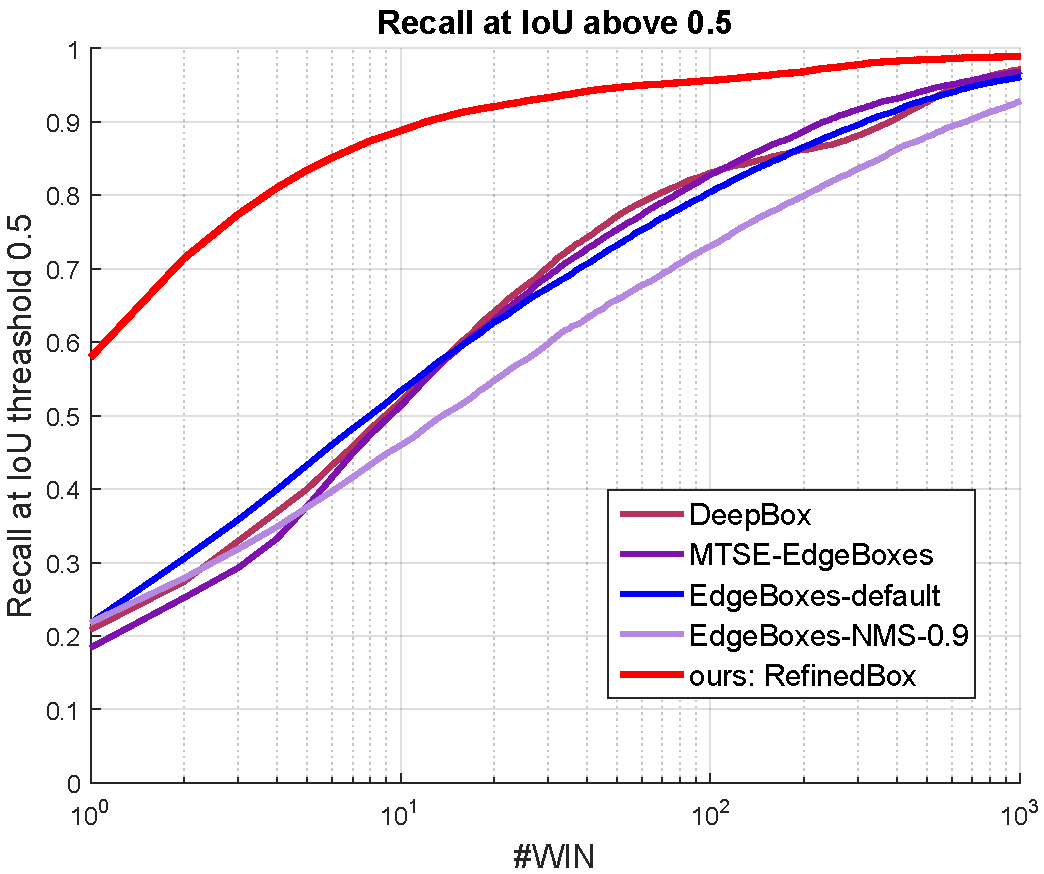
\includegraphics[width=.425\linewidth]{refine-recall-proposals-0_5} 
  \hspace{.03\linewidth}
  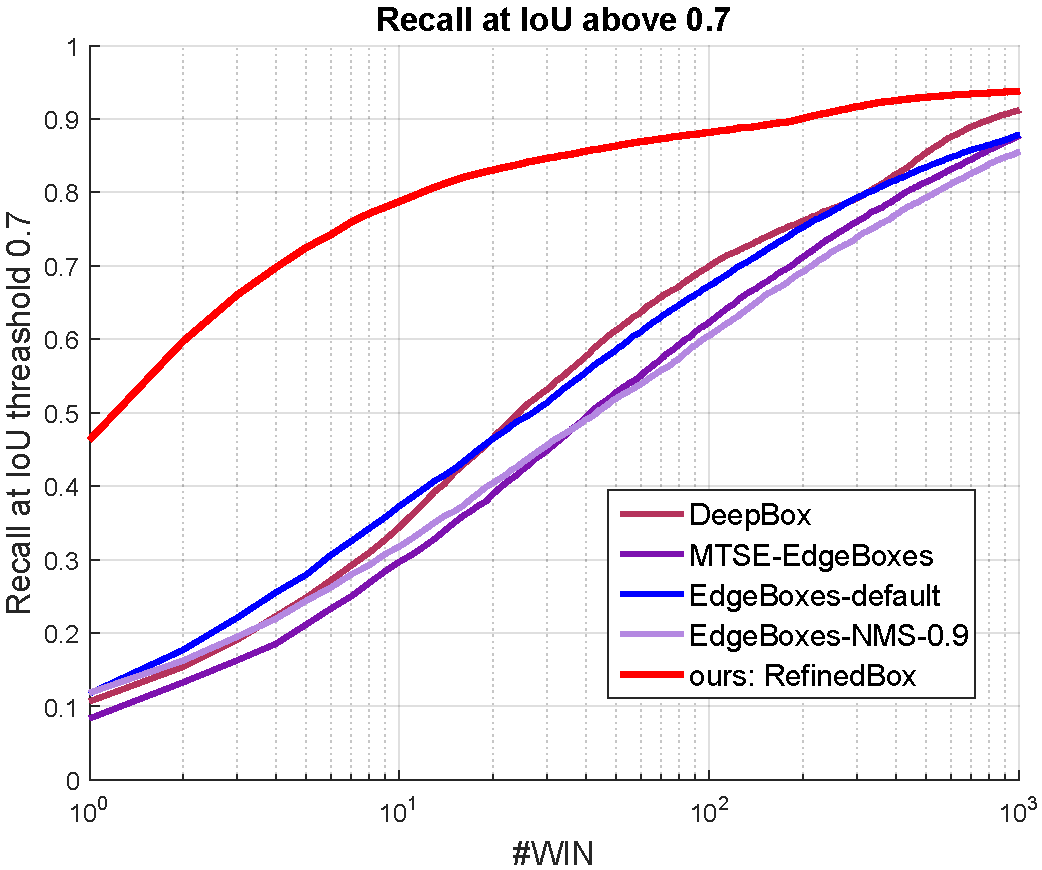
\includegraphics[width=.425\linewidth]{refine-recall-proposals-0_7} \\
  \caption{The evaluation of different refinement algorithms. 
  	These two subfigures show object detection recall \vs the 
    number of proposals (\#WIN) at IoU threshold 0.5 (left) and
    0.7 (right), respectively. The method of EdgeBoxes-default 
    is Edge Boxes \cite{zitnick2014edge} with default parameters, 
    and EdgeBoxes-NMS-0.9 changes the parameter of non-maximum 
    suppression (NMS) to 0.9.}
  \label{fig:refine-evaluation}
  \vspace{-0.15in}
\end{figure*}


\subsection{Joint Training with Object Detection} \label{sec: detection}
%
So far we have described how to train the proposal refinement network.
Since the proposed network is very lightweight,
it has the potential to share convolutional features 
with high-level applications.
Here, we use object detection as an example to show the joint 
training process of RefinedBox and consequent applications.
%
In order to test the ability of RefineBox to generate a few proposals
with high quality, we only use the top 10 proposals per image of RefinedBox 
to perform object detection.


As shown in \figref{fig:network}, we connect the well-known detection framework,
Fast R-CNN \cite{girshick2015fast}, after the convolutional layers as a parallel
branch to RefinedBox.
The refined proposals produced by the RefinedBox branch are inputted into Fast R-CNN.
%
In order to make the RefinedBox and Fast R-CNN share the same convolutional features,
we apply an alternating fine-tuning process.
The algorithm is presented in \algref{alg:training}.
After the alternating training, both networks form a unified network.
%
For each proposal box, there are 120.0 million FLOPs for the fully 
connected layers of the Fast R-CNN branch, while only 3.2 million 
FLOPs for the fully connected layers of the RefinedBox branch.
Thus, the RefinedBox branch only incurs a little extra computational load.


For the training of the detection module, each mini-batch has 256 
object proposals that are from the same image.
As in Fast R-CNN \cite{girshick2015fast}, 25\% of these proposals 
have IoU overlap with a ground truth of at least 0.5, and they are 
viewed as positive samples.
The remaining negative samples have max IoU overlap with ground truth
in the interval [0.1, 0.5).
The top 1000 proposals generated by RefinedBox are used in training.
The learning rate is 1e-3 for the first 50k iterations of SGD,
and then the learning rate is divided by 10 for another 20k iterations.
For test, only the top 10 proposals (per image) of RefinedBox are used.
In contrast, the traditional proposal methods, such as Edge Boxes and
Selective Search, usually need thousands of proposals.



%%%%%%%%%%%%%%%%%%%%%%%%%%%%%%%%%%%%%%%%%%%%%%%%%%%%%%%%%%%%%%%%%%%%%%%%%%%%%%%
\section{Experiments}
%due to space constraints.
We evaluate our method on the widely used PASCAL VOC2007 dataset
\cite{pascal-voc-2007} which is composed of 2501 training, 2510 validation, and
4952 test images with corresponding annotations across 20 object categories.
All the experiments in this paper are trained on the VOC2007 \textit{trainval}
set and tested on the VOC2007 \textit{test} set.
% The input can also be replaced by other proposal
% generation methods since our method is generic for box refinement.
The experiments are conducted on a GTX TITAN X GPU using the publicly
available code \footnote{https://github.com/rbgirshick/py-faster-rcnn}.


Our experiments are divided into two parts.
The first part contains the comparison about object proposal, in which we
compare the existing mainstream proposal methods with ours in detail.
In the second part, we feed the proposals produced by these methods into a
region-based object detection framework, Fast R-CNN \cite{girshick2015fast},
to evaluate the quality of proposals in object detection.
Our experiments demonstrate that our method can generate high-quality
proposals for object detection with good efficiency.


\begin{figure*}[!htbp]
  \centering
  \subfloat[]{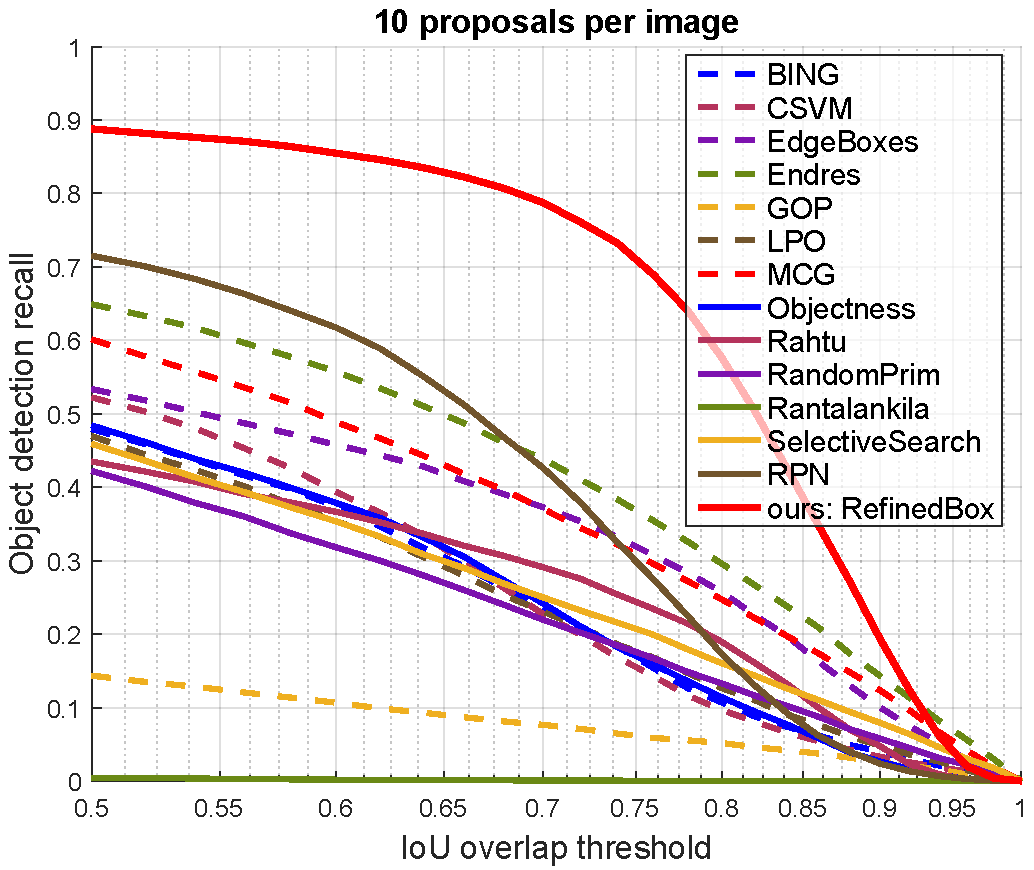
\includegraphics[width=.425\linewidth]{recall-threshold-10bb}}
  \hspace{.05\linewidth}
  \subfloat[]{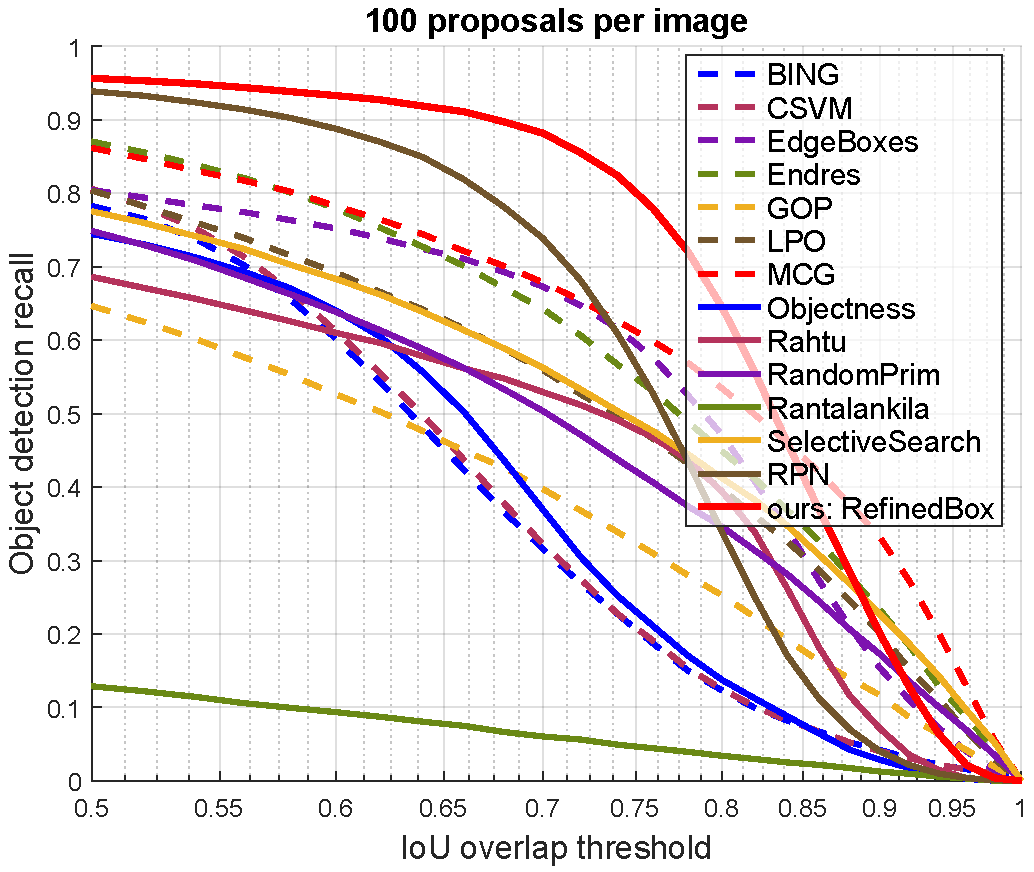
\includegraphics[width=.425\linewidth]{recall-threshold-100bb}}
  \\ \vspace{-0.1in}
  \subfloat[]{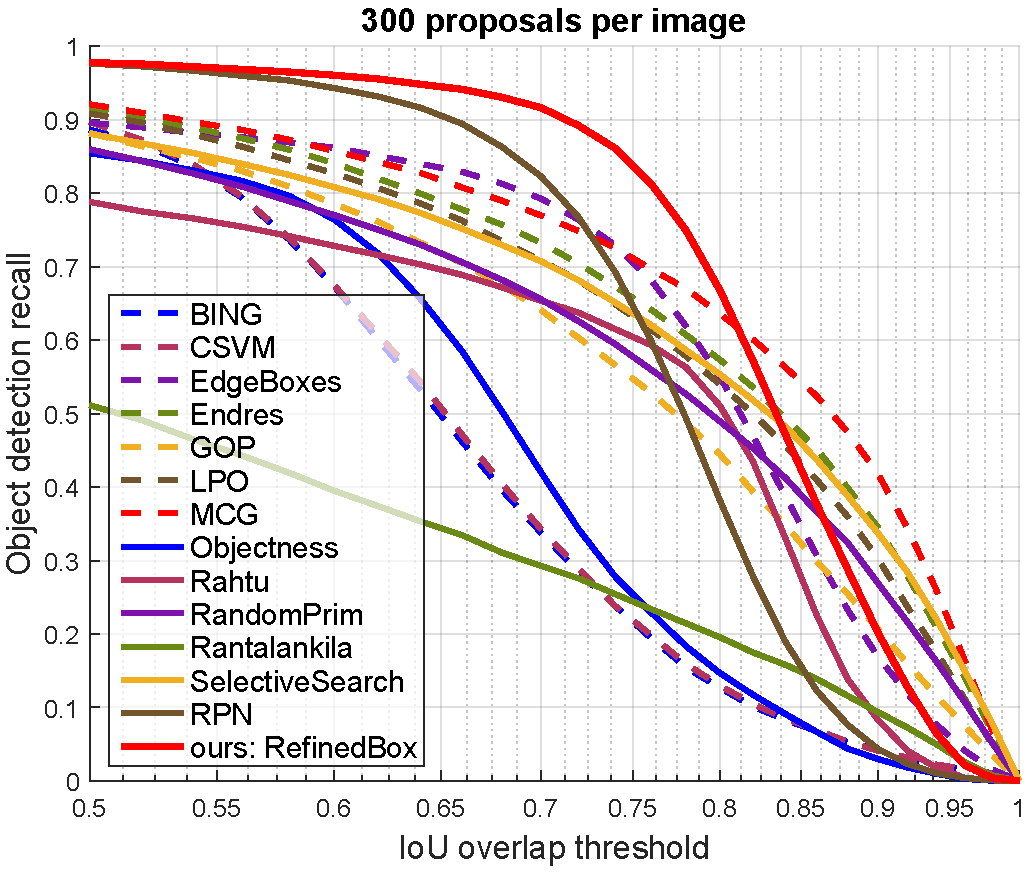
\includegraphics[width=.425\linewidth]{recall-threshold-300bb}}
  \hspace{.05\linewidth}
  \subfloat[]{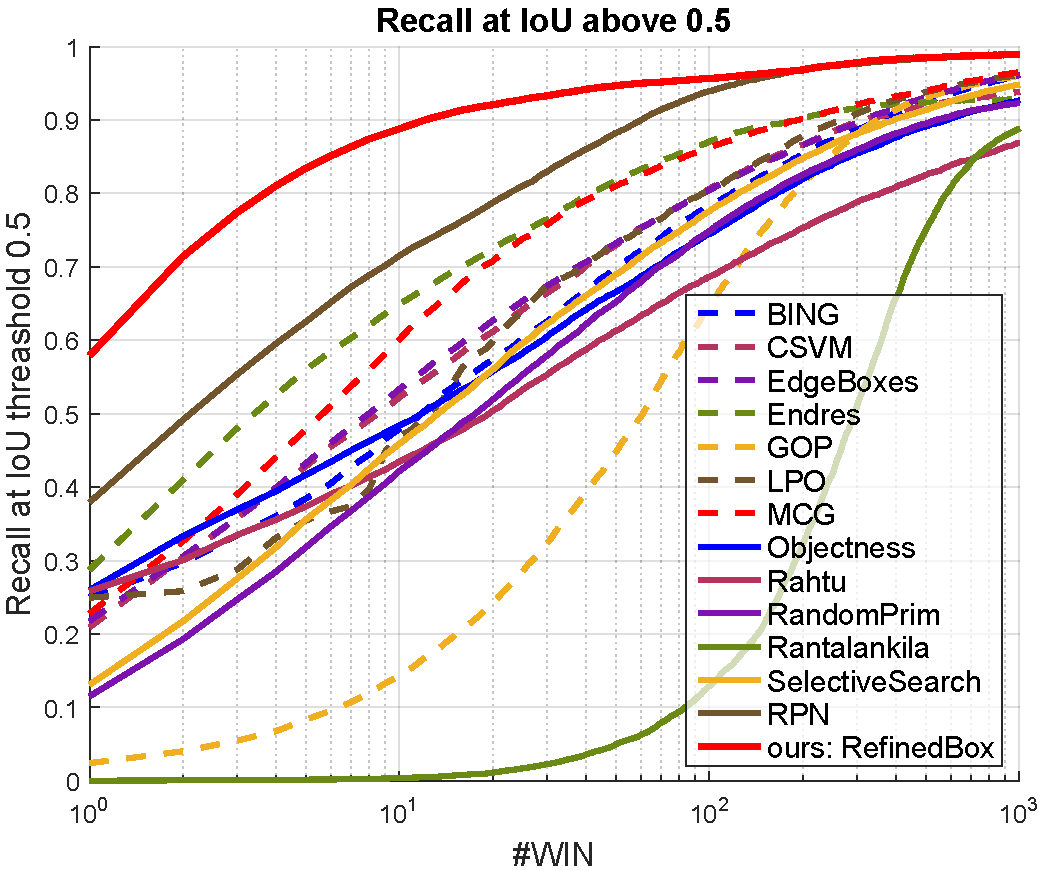
\includegraphics[width=.425\linewidth]{recall-proposals-0_5}}
  \\ \vspace{-0.1in}
  \subfloat[]{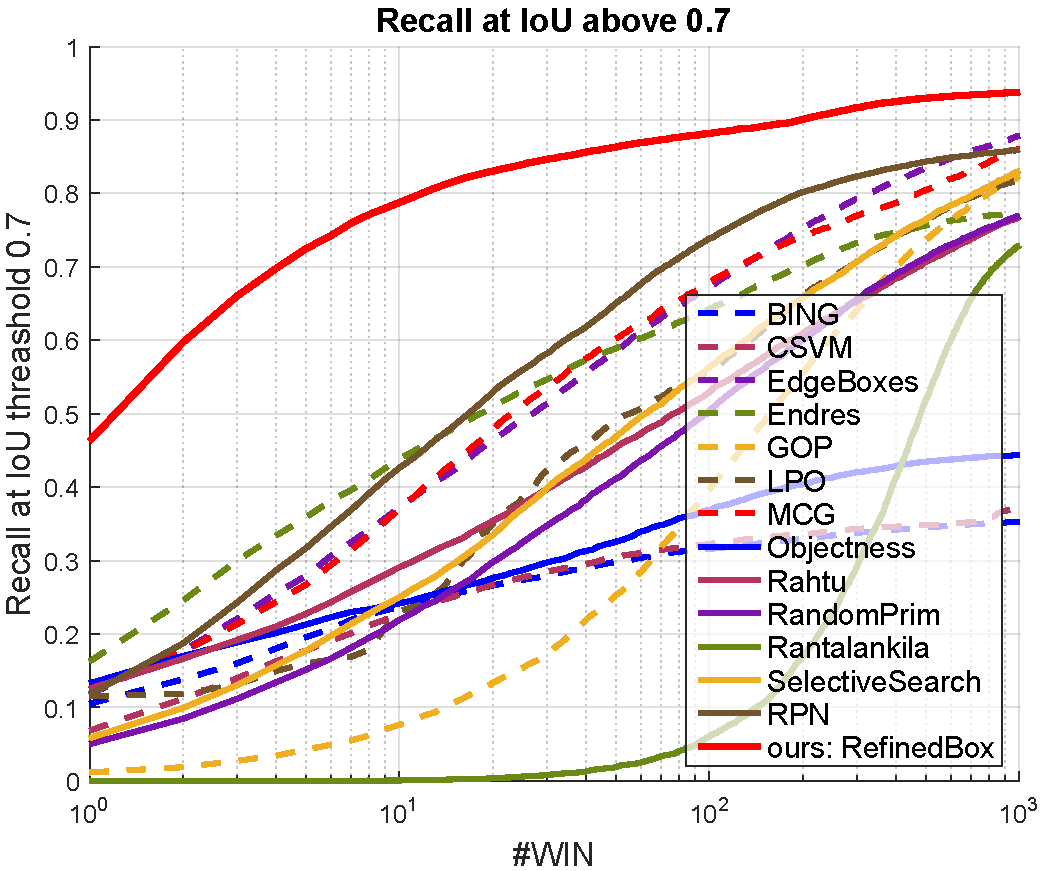
\includegraphics[width=.425\linewidth]{recall-proposals-0_7}}
  \hspace{.05\linewidth}
  \subfloat[]{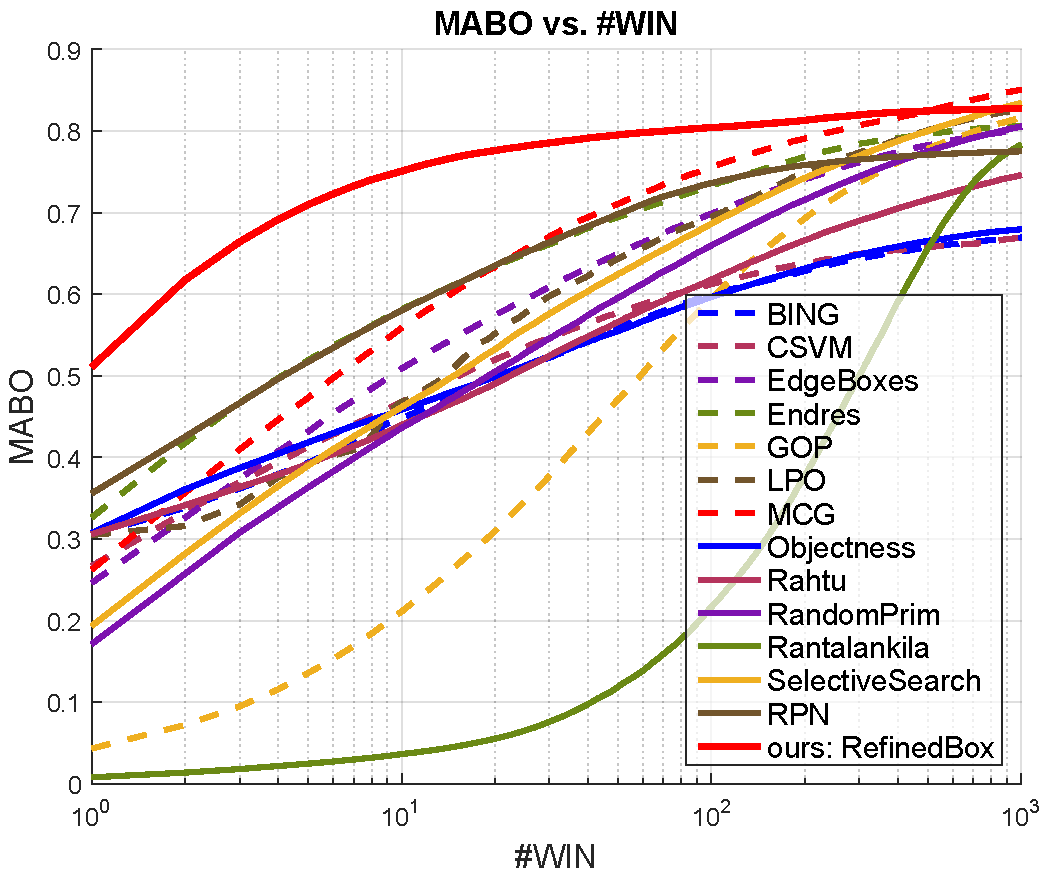
\includegraphics[width=.425\linewidth]{mabo-proposals}}
  \\ \vspace{-0.1in}
  \caption{The evaluation results on PASCAL VOC2007. (a)-(c) show object
  detection recall \vs IoU overlap threshold, using 10, 100, 300 proposals
  per image, respectively. (d)-(e) display object detection recall \vs the
  number of proposals (\#WIN) at IoU threshold 0.5 and 0.7, respectively.
  (f) shows MABO \vs the number of candidates using at most 1000 proposals
  per image.}
  \label{fig:voc-evaluation}
\end{figure*}


\subsection{Object Proposal Evaluation}
%
Here, we first compare our proposed RefinedBox with other proposal refinement
approaches such as DeepBox \cite{kuo2015deepbox} and MTSE \cite{chen2015improving}.
Then, we compare with some \sArt object proposal generation methods, including
Rahtu \cite{rahtu2011learning},
Objectness \cite{alexe2012measuring},
CSVM \cite{zhang2016object},
Selective Search \cite{uijlings2013selective},
RandomPrim \cite{manen2013prime},
Endres \cite{endres2014category},
Rantalankila \cite{rantalankila2014generating},
GoP \cite{krahenbuhl2014geodesic},
Edge Boxes \cite{zitnick2014edge},
BING \cite{cheng2014bing},
MCG \cite{arbelaez2014multiscale},
LPO \cite{krahenbuhl2015learning},
RPN \cite{ren2015faster}, and \etc.
% We take intersection-over-union (IoU) overlap scoring function as the
% measurement of the similarity between two bounding boxes.
% The IoU is the ration of intersection area of two bounding boxes and their union.
To evaluate the proposals, we adopt the metrics of object detection recall (DR),
average best overlap (ABO), and mean average best overlap (MABO).


\newcommand{\gEm}[1]{\underline{\bf #1}}
\newcommand{\tablefont}{\fontsize{8.2pt}{\baselineskip}\selectfont}
\newcommand{\tabincell}[2]{\begin{tabular}{@{}#1@{}}#2\end{tabular}}

\begin{table}[!b]
	\vspace{-0.2in}
    \centering
    \setlength\tabcolsep{2.8pt}
    \caption{The evaluation results (\%) on the VOC2007 \textit{test} set.
    RefinedBox$^1$, RefinedBox$^2$, RefinedBox$^3$ and RefinedBox$^4$ mean
    RefinedBox with Edge Boxes, MCG, Selective Search and RPN respectively.}
    \label{tab:voc-evaluation}
    \begin{tabular*}{\linewidth}{c|c|c|c|c|c|c|c} \hline
        \multirow{2}*{} & \multicolumn{3}{c|}{DR (IoU=0.5)}
        				& \multicolumn{3}{c|}{DR (IoU=0.7)}
             			& \multirow{2}*{\tabincell{c}{Time\\(s)}} \\ \cline{2-7}
        \diagbox{}{\#WIN} & 10 & 100 & 300  & 10 & 100 & 300  \\ \hline
        BING & 47.9 & 78.3 & 88.7 & 23.7 & 31.6 & 33.8 & \gEm{0.003} \\
        CSVM & 52.2 & 80.6 & 89.7 & 22.8 & 32.3 & 34.3 & 0.33 \\
        EdgeBoxes & 53.4 & 80.4 & 89.6 & 37.3 & 67.3 & 79.3 & 0.25 \\
        Endres & 64.9 & 87.1 & 91.6 & 43.9 & 64.3 & 73.3 & 19.94 \\
        GOP & 14.3 & 64.7 & 88.2 & 7.6 & 39.7 & 64.1 & 0.29 \\
        LPO & 47.0 & 80.4 & 90.9 & 23.1 & 56.0 & 70.9 & 0.46 \\
        MCG & 60.1 & 86.2 & 92.1 & 37.1 & 67.9 & 77.0 & 17.46 \\
        Objectness & 48.4 & 74.5 & 85.5 & 24.2 & 36.9 & 42.0 & 0.91 \\
        Rahtu & 43.5 & 68.6 & 78.8 & 29.1 & 52.9 & 65.4 & 0.67 \\
        RandomPrim & 42.2 & 74.9 & 86.0 & 22.0 & 50.4 & 65.6 & 0.12 \\
        Rantalankila & 0.4 & 12.9 & 51.1 &  0.1 & 6.0 & 29.3 & 3.57 \\
        SelectiveSearch & 45.9 & 77.6 & 88.1 & 25.0 & 56.3 & 70.7 & 1.60 \\
        RPN & 71.5 & 93.9 & 97.7 & 42.6 & 73.9 & 82.3 & 0.10 \\ \hline
        RefinedBox$^1$ & \gEm{88.8} & \gEm{95.7} & \gEm{97.8} & \gEm{78.8}
        	& \gEm{88.2} & \gEm{91.7} & 0.31 \\
        RefinedBox$^2$ & 88.3 & 94.9 & 97.4 & 78.1 & 85.0 & 88.1 & 17.52 \\
        RefinedBox$^3$ & 87.9 & 93.5 & 95.6 &  \gEm{78.8} & 85.5 & 88.2 & 1.66 \\
        RefinedBox$^4$ & \gEm{88.8} & 95.5 & 97.2 & 76.5 & 85.9 & 89.6
        	& 0.16 \\ \hline
    \end{tabular*}
\end{table}


\begin{table*}[!htbp]
    \centering
    \setlength\tabcolsep{1.4pt}
    \caption{The ABO \& MABO (\%) of various competitors using 300 proposals 
    	per image on the VOC2007 \emph{test} set. RefinedBox$^1$, 
        RefinedBox$^2$, RefinedBox$^3$ and RefinedBox$^4$ mean RefinedBox 
        with Edge Boxes, MCG, Selective Search and RPN respectively.}
    \label{tab:voc-mabo}
    \begin{tabular*}{\textwidth}{c|cccccccccccccccccccc|c} \hline
        Methods & aer. & bic. & bird & boat & bot. & bus & car & cat & cha.
        & cow & din. & dog & hor. & mot. & per. & pot. & she. & sofa & tra.
        & tv & mAP\\ \hline
        %
        BING&60.4&63.9&60.0&56.1&48.7&64.2&57.4&70.2&60.8&61.0&
        68.7&67.5&64.6&64.3&58.5&56.8&59.0&68.5&68.0&59.6&61.9\\
        %
        CSVM&66.1&64.1&61.0&60.1&54.2&66.8&61.6&68.8&60.4&63.6&
        65.9&66.7&65.1&64.5&57.4&56.4&61.6&67.8&68.2&59.1&63.0\\
        %
        EdgeBoxes&75.3&77.3&72.3&71.6&52.3&81.4&69.3&80.2&66.3&79.1
        &76.9&81.8&79.5&76.3&64.8&60.2&75.6&80.1&78.1&77.4&73.8\\
        %
        Endres&70.4&77.0&71.5&65.5&57.0&81.8&76.5&\gEm{87.4}&69.6
        &77.3&\gEm{83.0}&\gEm{85.9}&80.3&79.1&67.6&65.0&74.3&
        \gEm{88.3}&82.1&76.1&75.8\\
        %
        GOP&68.3&70.2&69.0&66.7&54.7&77.5&72.4&79.4&66.4&76.5&
        73.7&78.1&69.3&69.5&64.6&59.2&72.9&79.9&73.7&78.3&71.0\\
        %
        LPO&73.8&74.0&71.1&69.6&51.6&81.2&74.2&86.6&67.1&78.9&
        79.9&84.2&77.0&76.3&65.3&62.6&75.8&84.6&80.4&75.6&74.5\\
        %
        MCG&75.4&77.9&73.0&68.6&63.3&84.7&75.3&87.2&72.3&80.2&
        82.3&85.1&81.0&78.1&72.4&66.3&76.6&87.6&\gEm{82.5}&\gEm{81.7}&77.6\\
        %
        Objectness&59.7&62.4&58.4&57.0&45.7&67.4&56.6&71.9&55.9&60.6
        &71.2&69.7&67.6&63.4&56.7&52.5&58.5&71.1&69.4&57.8&61.7\\
        %
        Rahtu&68.3&68.5&58.9&63.1&37.7&74.9&61.6&77.1&52.2&66.4&
        76.3&74.7&73.2&68.0&55.6&48.7&60.2&76.6&76.1&68.1&65.3\\
        %
        RandomPrim&76.5&72.8&68.1&69.3&51.1&76.7&68.1&83.5&66.5&73.3
        &82.5&80.8&73.6&73.8&62.0&58.4&67.6&84.3&75.6&72.5&71.8\\
        %
        Rantalankila&55.0&50.2&47.1&55.4&28.7&53.5&47.2&51.9&38.0&
        59.7&35.8&54.2&52.4&48.4&38.4&38.3&59.7&45.0&57.9&44.4&48.1\\
        %
        SelectiveSearch&77.0&75.3&71.5&68.3&51.8&79.2&69.7&86.1&66.8
        &74.1&\gEm{83.0}&85.1&77.1&75.5&64.1&61.4&69.2&85.9&79.6&74.8&73.8\\
        %
        RPN&70.5&76.9&73.0&70.3&67.4&74.9&75.8&77.9&72.9&78.1
        &76.1&78.1&77.3&75.8&75.2&68.4&74.8&76.9&76.1&74.6&74.6\\ \hline
        %
        RefinedBox$^1$&76.8&\gEm{81.5}&\gEm{77.8}&\gEm{77.3}&\gEm{71.0}
        &\gEm{85.9}&\gEm{82.3}&84.1&76.4&\gEm{82.6}&78.3&83.3&\gEm{82.0}
        &\gEm{81.3}&\gEm{79.2}&71.7&\gEm{80.2}&82.1&81.5&80.4&\gEm{79.8}\\
        %
        RefinedBox$^2$&76.0&81.2&76.5&73.9&69.1&85.6&81.8&83.2&\gEm{76.8}&
        81.2&80.4&82.8&81.8&80.1&77.9&\gEm{72.8}&79.5&83.5&82.2&81.4&79.4\\
        %
        RefinedBox$^3$&\gEm{78.3}&80.0&74.4&74.7&65.4&84.6&81.0&82.8&72.5&
        81.8&77.2&82.9&81.6&79.5&78.0&66.9&78.5&82.3&80.4&77.1&78.0\\
        RefinedBox$^4$&72.1&79.5&75.6&71.2&69.1&82.3&80.4&83.1&75.5&
        80.0&77.9&81.6&80.7&79.0&78.0&70.2&79.1&81.0&78.5&78.5&77.7\\ \hline
    \end{tabular*}
\end{table*}



The comparison between different proposal refinement approaches is shown
in \figref{fig:refine-evaluation}.
We choose Edge Boxes \cite{zitnick2014edge} to produce the initial proposals
which are inputted into these refinement algorithms, but we change the default
parameter of non-maximum suppression from 0.75 to 0.9 in order to obtain more boxes.
% The method of EdgeBoxes-default uses the default parameters of EdgeBoxes,
% while the EdgeBoxes-NMS-0.9 changes the NMS threshold to 0.9.
We find that our method achieves much higher object detection recall than other
competitors at both IoU thresholds 0.5 and 0.7.
The gap between our RefinedBox and other competitors is very large.
Using only one proposal per image, RefinedBox achieves a detection recall of
57.9\% and 46.3\% at IoU 0.5 and IoU 0.7, respectively.
In addition, RefinedBox can share the convolutional layer with subsequent object
detection and the additional layers of RefinedBox are computationally lightweight,
so RefinedBox is an efficient detection framework.
In fact, the total time consumption of RefinedBox and subsequent object detection
is similar to the Faster R-CNN \cite{ren2015faster} at about 0.13 second per image.
DeepBox builds a separate network to re-rank boxes,
while MTSE segments an image first and then uses superpixels to refine boxes;
however, the image segmentation step is a time-consuming operation.
Thus, RefinedBox is more suitable to be used in high-level applications.


Extensive comparisons with other object proposal generation methods
are shown in \figref{fig:voc-evaluation}.
RefinedBox also uses Edge Boxes as input,
and we apply the default parameters for the evaluation of Edge Boxes.
Our method achieves the \sArt performance across all cases.
%
% We also observe that the detection recall of RPN drops sharply for high IoU
% thresholds.
% Although RefinedBox also suffers a drop for high IoU thresholds,
% it always performs better than RPN and EdgeBoxes.
% We believe that this is due to the initial input boxes
% and that this problem can be overcome if some other proposal generation methods are used.
%
For object detection recall \vs the number of proposals at IoU 0.7,
the performance improvements between RefinedBox and other competitors are also very large.
The higher detection recall and fewer proposals will benefit the subsequent
high-level applications a lot.
%
RPN has recently become popular for object detection,
but our proposed RefinedBox is much more accurate than it.
The object detection recall of RefinedBox with only 10 proposals per image
is similar to RPN using 100 proposals per image.
The improvement from RPN to RefinedBox demonstrates the effectiveness of our method.
%
With only a small number of proposals,
RefinedBox can achieve much better performance than other competitors.
Using only 30 proposals, RefinedBox can achieve detection recall of
93.3 and 84.7 for IoU overlap 0.5 and 0.7, respectively.
This will meet the requirements of many applications for a small amount
of but high-quality object proposals.


To quantify these plots, we list the corresponding numbers
in \tabref{tab:voc-evaluation}.
RefinedBox achieves much better performance than various initial
input methods.
With Edge Boxes and an IoU threshold of 0.5, the detection recall of 
RefinedBox is 17.3\%, 1.8\%, and 0.1\% higher than the second place 
method (RPN) when using 10, 100, and 300 proposals per image, respectively.
At an IoU threshold of 0.7, the detection recall of RefinedBox with EdgeBoxes
is 36.2\%, 14.3\% and 9.4\% higher than RPN when 10, 100 and 300 proposals
are used per image respectively.
Since our goal is to significantly reduce the number of proposals,
the evaluation results suggest that we have achieved it.
% Using 300 proposals per image, the MABO of RefinedBox is 1.3\% higher than
% MCG, which achieves the second place on this metric.
We also notice that RPN is much better than other competitors except RefinedBox.
This is the key reason why Faster R-CNN can achieve better detection performance
than Fast R-CNN.
The runtime of RefinedBox for each image is about 0.06 second,
which is very fast when compared with these bottom-up proposal generation methods.
% EdgeBoxes and MCG achieve the \sArt performance among non-deep learning
% based methods.
% That is why we choose EdgeBoxes as the input of RefinedBox.
%
We report the ABO and MABO of various competitors in \tabref{tab:voc-mabo}.
As expected, RefinedBox achieves the best performance again.


% \begin{table*}[!htbp]
%     \centering
%     \setlength\tabcolsep{1.4pt}
%     \caption{Detection average precision (\%) using Fast R-CNN on the VOC2007
%     	\emph{test} set. RefinedBox$^1$, RefinedBox$^2$, RefinedBox$^3$ and
%         RefinedBox$^4$ mean RefinedBox with Edge Boxes, MCG, Selective Search 
%         and RPN respectively.}
%     \label{tab:voc-detection}
%     \begin{tabular*}{\textwidth}{c|cccccccccccccccccccc|c} \hline
%         Methods & aer. & bic. & bird & boat & bot. & bus & car & cat & cha.
%         & cow & din. & dog & hor. & mot. & per. & pot. & she. & sofa & tra.
%         & tv & mAP\\ \hline
%         %
%         BING&65.0&68.6&61.8&46.8&42.2&72.1&71.4&77.7&31.4&69.7
%             &56.3&74.0&75.7&66.3&65.4&27.1&62.1&60.6&68.7&60.0&61.2\\
%         %
%         CSVM&68.0&71.3&60.3&44.1&33.7&73.0&69.1&77.1&28.7&68.1
%             &58.7&71.5&78.3&69.5&60.7&25.6&57.4&61.4&72.5&55.7&60.2\\
%         %
%         EdgeBoxes&\gEm{73.4}&78.1&68.4&55.7&39.2&79.5&76.8&81.0&41.7&73.7
%         		 &65.6&82.8&82.6&76.2&68.1&34.8&66.2&70.1&77.1&58.9&67.5\\
%         %
%         Endres&63.3&75.0&63.4&43.0&31.2&77.2&70.5&78.1&32.8&66.8
%               &67.6&75.3&78.7&70.9&61.1&28.0&61.6&66.3&75.9&61.3&62.4\\
%         %
%         GOP&67.2&76.3&65.7&51.5&32.4&78.4&78.6&81.1&40.7&74.1
%            &64.2&78.7&80.5&74.3&67.3&30.7&65.4&\gEm{70.6}&76.5&66.1&66.0\\
%         %
%         LPO&67.4&76.9&\gEm{68.8}&52.1&30.4&81.3&75.0&79.9&37.9&73.9
%            &67.6&76.4&80.3&70.1&66.1&33.5&65.0&68.0&76.4&63.9&65.6\\
%         %
%         MCG&69.8&77.2&67.2&51.8&42.5&80.0&76.8&78.6&43.9&71.4
%            &68.1&77.1&81.5&70.9&67.8&33.0&65.5&68.2&77.1&64.8&66.7\\
%         %
%         Objectness&64.7&73.5&60.4&40.1&34.8&72.7&69.5&76.8&31.5&67.4
%         		  &59.0&77.7&79.1&71.4&60.8&30.5&54.6&62.0&73.5&57.5&60.9\\
%         %
%         Rahtu&69.2&68.6&59.1&53.8&23.1&78.4&67.2&79.9&26.9&66.6
%         	 &68.5&76.7&79.7&70.3&58.0&26.9&57.1&64.2&77.2&60.5&61.6\\
%         %
%         RandomPrim&69.8&78.4&61.5&52.6&25.3&76.0&69.3&78.3&39.2&67.5&\gEm{69.8}
%         	      &76.2&\gEm{82.7}&69.5&58.8&27.6&53.7&67.5&76.3&58.5&62.9\\
%         %
%         Rantalankila&68.0&67.7&63.1&42.3&21.5&71.5&64.5&78.7&29.8&69.2
%         			&67.6&74.3&77.1&66.9&54.7&25.2&60.6&63.8&75.9&59.9&60.1\\
%         %
%         SelectiveSearch&72.9&78.3&66.0&54.3&34.7&81.3&76.8&83.3&41.5&74.5&66.4
%         			   &79.8&82.2&76.2&65.5&35.2&65.6&70.1&\gEm{77.4}&65.9&67.4\\
%         %
%         RPN&67.5&78.5&67.3&51.9&51.5&76.2&79.8&84.4&50.2&74.3&66.9&\gEm{83.2}
% 		   &80.0&73.9&76.5&37.1&\gEm{69.4}&65.7&76.5&74.2&69.2 \\ \hline
%         %
%         RefinedBox$^1$&70.0&79.7&66.4&58.8&\gEm{58.0}&78.3&80.0
%         	&\gEm{86.4}&52.2&73.7&\gEm{69.8}&81.4&80.6&75.9&77.6
%             &\gEm{46.5}&68.1&67.8&76.7&73.1&\gEm{71.1} \\
%         RefinedBox$^2$&68.6&\gEm{80.1}&67.5&55.0&55.5&79.2&79.4&79.7&51.6&75.3&
%         65.8&76.7&80.7&76.9&77.4&41.3&68.5&69.8&\gEm{77.4}&\gEm{74.8}&70.1\\
%         RefinedBox$^3$&68.1&78.2&67.7&\gEm{59.5}&56.4&83.4&\gEm{80.3}&79.4&\gEm{52.9}
%         &75.1&\gEm{69.8}&77.2&80.4&76.2&\gEm{78.2}&42.0&69.0&69.4&76.1&73.7&70.7\\
%         RefinedBox$^4$&68.6&79.4&68.2&55.6&56.1&\gEm{84.0}&80.2&84.1&52.8&\gEm{75.5}
%     	&\gEm{69.8}&77.8&80.6&\gEm{77.1}&78.1&43.9&67.3&65.6&75.8&72.8&70.7\\ \hline
%     \end{tabular*}
% \end{table*}


\begin{table*}[!htbp]
    \centering
    \setlength\tabcolsep{1.4pt}
    \caption{Detection performance (\%) using only 10 proposals per image on the VOC2007
    	\emph{test} set. RefinedBox$^1$, RefinedBox$^2$, RefinedBox$^3$ and
        RefinedBox$^4$ mean RefinedBox with Edge Boxes, MCG, Selective Search 
        and RPN, respectively.}
    \label{tab:voc-detection}
    \begin{tabular*}{\textwidth}{c|cccccccccccccccccccc|c} \hline
        Methods & aer. & bic. & bird & boat & bot. & bus & car & cat & cha.
        & cow & din. & dog & hor. & mot. & per. & pot. & she. & sofa & tra.
        & tv & mAP\\ \hline
        %
        BING&36.8&34.9&33.4&25.4&9.1&44.7&34.5&61.4&10.3&25.1
        &34.3&55.1&59.6&42.2&25.5&13.8&17.5&45.8&55.2&23.5&34.4\\
        %
        CSVM&51.5&42.3&35.1&26.6&9.1&52.4&35.9&61.7&10.7&23.8
        &30.3&52.7&62.0&43.1&25.7&9.8&18.6&40.7&58.6&23.9&35.7\\
        %
        EdgeBoxes&52.4&43.5&40.2&37.4&9.1&60.4&39.3&55.0&10.3&40.0
        &32.2&54.3&60.7&46.1&24.7&10.9&34.1&34.2&62.0&35.2&39.1\\
        %
        Endres&53.7&44.7&47.4&29.4&9.1&57.4&44.8&73.5&13.4&42.8
        &34.3&63.9&67.1&53.0&32.8&14.4&33.2&50.1&64.5&26.0&42.8\\
        %
        GOP&26.6&9.1&21.9&16.7&9.1&9.1&9.2&19.6&9.1&20.6
        &0.0&15.6&9.1&9.1&9.1&4.5&20.1&10.3&13.9&22.9&13.3\\
        %
        LPO&51.7&34.8&33.3&25.5&9.1&50.7&36.2&61.5&10.3&33.0
        &28.4&51.0&50.1&40.8&22.4&9.5&24.4&36.8&59.5&21.9&34.5\\
        %
        MCG&49.6&42.5&42.3&28.2&15.0&54.1&41.7&69.7&14.0&46.3&
        24.3&61.2&61.1&46.3&32.5&13.1&39.7&46.1&57.5&37.8&41.2\\
        %
        Objectness&41.4&41.7&33.3&24.1&9.1&49.3&35.7&60.3&10.5&24.0
        &32.8&57.4&57.5&42.4&25.4&13.2&18.4&42.6&56.7&22.4&34.9\\
        %
        Rahtu&46.9&34.2&26.8&24.5&9.1&46.8&34.5&62.0&7.6&22.8
        &31.0&50.4&49.5&41.0&20.5&11.4&17.5&35.1&52.6&23.3&32.4\\
        %
        RandomPrim&46.8&36.1&33.0&24.8&9.1&41.7&33.1&60.3&10.0&23.7
        &29.2&48.6&46.1&34.3&20.1&11.5&17.4&38.5&50.0&22.7&31.9\\
        %
        Rantalankila&0.0&0.0&1.5&0.3&0.8&0.0&2.3&0.0&2.3
        &9.1&0.0&9.1&0.0&0.0&4.5&4.5&9.1&0.0&0.0&5.2&2.4\\
        %
        SelectiveSearch&46.6&36.2&33.6&25.0&9.1&46.6&35.4&61.5&11.4
        &23.9&31.9&49.8&50.9&41.8&23.9&12.8&18.1&43.5&57.1&22.1&34.1\\
        %
        RPN&59.9&59.8&51.5&44.7&32.0&60.9&62.7&71.2&28.7&66.4&\gEm{58.8}
        &70.1&71.8&51.6&53.3&22.3&52.4&51.6&69.0&44.0&54.1 \\ \hline
        %
        RefinedBox$^1$&\gEm{70.2}&71.9&60.1&54.8&\gEm{43.6}&78.1
        &72.1&\gEm{80.0}&46.0&68.1&56.9&77.6&79.6&\gEm{70.8}&70.4
        &\gEm{37.9}&61.3&63.4&77.7&67.9&65.4 \\
        %
        RefinedBox$^2$&62.1&\gEm{72.1}&61.0&54.0&42.9&\gEm{79.3}
        &72.0&79.5&\gEm{46.5}&67.7&58.7&\gEm{77.7}&\gEm{80.6}
        &70.5&70.4&36.3&\gEm{61.6}&63.6&\gEm{77.9}&\gEm{68.8}&65.2 \\
        %
        RefinedBox$^3$&68.9&71.3&60.5&\gEm{56.0}&41.8&79.2
        &\gEm{72.2}&79.8&46.4 &\gEm{70.1}&\gEm{58.8}&77.0&80.1
        &70.3&70.4&37.2&61.3&\gEm{64.9}&75.5&68.3&\gEm{65.5} \\
        %
        RefinedBox$^4$&67.3&71.6&\gEm{68.0}&52.4&42.3&76.9
        &72.1&79.0&\gEm{46.5}&69.0&54.8&77.3&80.0&70.1&\gEm{70.7}
        &36.0&60.9&61.2&74.8&68.0&65.0 \\ \hline
    \end{tabular*}
\end{table*}


\begin{figure*}[!t]
  \centering
  \newcommand{\AddImg}[1]{\includegraphics[height=.143\linewidth]{Ilu/#1.png}}
  \AddImg{000038}\hfill \AddImg{000062}\hfill \AddImg{000069}\hfill
  \AddImg{000071}\hfill \AddImg{000076}
  \\ \vspace{.03in}
  \renewcommand{\AddImg}[1]{\includegraphics[height=.198\linewidth]{Ilu/#1.png}}
  \AddImg{000010}\hfill \AddImg{003041}\hfill \AddImg{003572}\hfill
  \AddImg{009547}\hfill \AddImg{003854}\hfill \AddImg{003976}\hfill
  \AddImg{006640}
  \\ \vspace{.03in}
  \renewcommand{\AddImg}[1]{\includegraphics[height=.139\linewidth]{Ilu/#1.png}}
  \AddImg{000124}\hfill \AddImg{000319}\hfill \AddImg{000570}\hfill
  \AddImg{003647}\hfill \AddImg{005080}
  \\
  \caption{Some detection samples of our RefinedBox method. 
  Note that only the top 10 proposals per image are used.
  All images are from VOC2007 \textit{test} set.}
  \label{fig:visual}
  \vspace{-0.008in}
\end{figure*}



\subsection{Object Detection}
%
% Since object proposal generation aims to provide proposals
% for consequent object detection, the quality of proposals
% needs to be tested in object detection.
%
Since object detection is an important application of object
proposals, we test the quality of different proposal algorithms
according to their performance in object detection.
%
We feed the proposals produced by the aforementioned
methods into a well-known region-based object detection framework,
Fast R-CNN \cite{girshick2015fast}.
We optimize RefinedBox using the joint training algorithm described above.
%For RPN, we simply test Faster R-CNN \cite{ren2015faster}.
%For other bottom-up methods, 
We follow the settings in \cite{zhang2017sequential}.
The top 1000 proposals per image are used to retrain the Fast R-CNN
network.
All of these methods are trained on the VOC2007 \textit{trainval} set
and tested on the \textit{test} set.
Note that only the top 10 proposals per image are used to evaluate 
the ability of generating a small amount of proposals for different
methods.


The results are summarized in \tabref{tab:voc-detection}.
In terms of mAP, RefinedBox is 26.3\%, 24.0\%, 31.4\% and 
10.9\% higher than the original proposal methods, \ie
Edge Boxes, MCG, Selective Search and RPN, respectively.
% These evaluation results demonstrate the effectiveness of RefinedBox
% in object detection.
% Since RefinedBox can be embedded into a detection network as a
% computationally lightweight branch, it has the potential to significantly
% improve object detection.
Compared with other proposal generation methods, RefinedBox can also
achieve much higher detection performance.
These evaluation results demonstrate that RefinedBox can generate
a small amount of proposals with significantly high quality.
We display some detection examples produced by RefinedBox in \figref{fig:visual}.



%%%%%%%%%%%%%%%%%%%%%%%%%%%%%%%%%%%%%%%%%%%%%%%%%%%%%%%%%%%%%%%%%%%%%%%%%%%%%%%
\section{Conclusion}
%
In this paper, we present a proposal refinement
method using re-ranking and box regression.
%
It is very efficient because the added layers are designed
to be computationally lightweight.
% Extensive experiments demonstrate that RefinedBox can achieve
% high detection recall with only a small amount of object proposals.
% Thus RefinedBox can significantly reduce the number of proposals
% generated by previous algorithms.
Extensive experiments demonstrate that RefinedBox can significantly 
reduce the number of proposals generated by previous algorithms.
Since the refinement network can be easily optimized,
we find we can perform joint training of it with consequent applications.
%
The evaluation on object detection demonstrates the effectiveness
of RefinedBox.
%
A small amount of but high-quality object proposals meet the requirements
of many high-level applications, including multi-label image classification,
\cite{wei2016hcp}, pedestrian detection \cite{paisitkriangkrai2016pedestrian},
deep multiple instance learning \cite{wu2015deep}, and \etc.
With fewer but more accurate proposals, these tasks are expected to achieve
better performance.
%
In the future, we plan to apply our refinement method to other 
high-level applications, \eg mining knowledge from huge amounts of unlabeled data.



{\small
\bibliographystyle{ieee}
\bibliography{RefinedBox}
}

\end{document} 